\documentclass{llncs}
\usepackage{etex}

\usepackage{amsmath,amssymb}
\usepackage{url}
\usepackage[linesnumbered,boxed,noline,noend]{algorithm2e}
\def\defaultHypSeparation{\hskip.1in}

\usepackage{graphicx}
\usepackage{subfig}

\usepackage{bussproofs}

\usepackage{logictools}
\usepackage{prooftheory}



\renewcommand{\topfraction}{0.85}
\renewcommand{\textfraction}{0.1}
\renewcommand{\floatpagefraction}{0.75}


\newcommand{\freevar}[1]{\mathrm{FV}(#1)}

\newcommand{\Vertices}[1]{V_{#1}}
\newcommand{\Edges}[1]{E_{#1}}
\newcommand{\Conclusion}[1]{\clause_{#1}}

\newcommand{\axiom}[1]{\widehat{#1}}
\newcommand{\n}{v}
\newcommand{\raiz}[1]{\rho(#1)}

\newcommand{\pedge}[3]{\ensuremath{\raiz{#1} \xrightarrow{#2} \raiz{#3}}}


\newcommand\inlineeqno{\stepcounter{equation}\ (\theequation)}



\newcommand{\con}[3]{\lfloor #1 \rfloor_{#2}^{#3}}


\newcommand{\res}[4]{\mathrel{\operatorname*{\odot}_{#1 #3}^{#2 #4}}}

\title{Towards the Compression of First-Order Resolution Proofs by Lowering Unit Clauses}

\author{
  Jan Gorzny\inst{1}
  \thanks{Supported by the Google Summer of Code 2014 program.}
  \and 
  Bruno Woltzenlogel Paleo\inst{2}
  \thanks{Stipendiat der \"Osterreichischen Akademie der Wissenschaften (APART).}
}

\authorrunning{J.\~Gorzny \and B.\~Woltzenlogel Paleo}

\institute{
  \email{jgorzny@uvic.ca}, University of Victoria, Canada
  \and 
  \email{bruno@logic.at}, Vienna University of Technology, Austria
}




\begin{document}

\maketitle


\begin{abstract}
The recently developed {\LowerUnits} algorithm compresses
propositional resolution proofs generated by SAT- and SMT-solvers by postponing and lowering resolution inferences involving unit clauses, which have exactly one literal. This paper describes a generalization of this algorithm to the case of first-order resolution proofs generated by automated theorem provers. An empirical evaluation of a simplified version of this algorithm on hundreds of proofs shows promising results.
\end{abstract}


\setcounter{footnote}{0}


\section{Introduction}

Most of the effort in automated reasoning so far has been dedicated to the design and implementation of proof systems and efficient theorem proving procedures. As a result, saturation-based first-order automated theorem provers have achieved a high degree of maturity, with resolution and superposition being among the most common underlying proof calculi. Proof production is an essential feature of modern state-of-the-art provers and proofs are crucial for applications where the user requires certification of the answer provided by the prover. Nevertheless, efficient proof production is 
non-trivial,
and it is to be expected that the best, most efficient, provers do not necessarily generate the best, least redundant, proofs. Therefore, it is a timely moment to develop methods that post-process and simplify proofs. While the foundational problem of simplicity of proofs can be traced back at least to Hilbert's 24th Problem, the maturity of automated deduction has made it particularly relevant today.  

For proofs generated by SAT- and SMT-solvers, which use propositional resolution as the basis for the DPLL and CDCL decision procedures, there is now a wide variety of proof compression techniques. Algebraic properties of the resolution
operation that might be useful for compression were investigated in \cite{bwp10}.

The {\ReduceReconstruct} algorithm \cite{RedRec} searches for locally redundant
subproofs that can be rewritten into subproofs of stronger clauses and with fewer resolution steps.
A linear time proof compression algorithm based on partial
regularization was proposed in \cite{RP08} and improved in \cite{LURPI}. Furthermore, \cite{LURPI} described a linear time algorithm called {\LowerUnits} that delays resolution with unit clauses.

In contrast, for first-order theorem provers, there has been up to now (to the best of our knowledge) no attempt to design and implement an algorithm capable of taking a first-order resolution DAG-proof and efficiently simplifying it, outputting a possibly shorter pure first-order resolution DAG-proof. There are algorithms aimed at simplifying first-order sequent calculus tree-like proofs, based on cut-introduction and Herbrand sequents \cite{BrunoLPAR,Hetzl,HerbrandSequent}. There is also an algorithm \cite{LPARCzech} that looks for terms that occur often in any TSTP \cite{TPTP} proof (including first-order resolution DAG-proofs) and introduces abbreviations for these terms. However, as the definitions of the abbreviations are not part of the output proof, it cannot be checked by a pure first-order resolution proof checker.

In this paper, we initiate the process of lifting propositional proof compression techniques to the first-order case, starting with the simplest known algorithm: {\LowerUnits} (described in \cite{LURPI}). 
As shown in Section \ref{sec:Challenges}, even for this simple algorithm, the fact that first-order resolution makes use of unification leads to many challenges that simply do not exist in the propositional case. In Section \ref{sec:SimpleFOLU} we describe an easy to implement algorithm with  linear time complexity (with respect to the proof length) which partially overcomes these challenges. 
In Section \ref{sec:exp} we present experimental results obtained by applying this algorithm on hundreds of proofs generated with the{\
SPASS} theorem prover. 
The next section introduces the first-order resolution calculus using notations that are more convenient for describing proof transformation operations.





\section{The Resolution Calculus}

We assume that there are infinitely many variable symbols (e.g. $X$, $Y$, $Z$, $X_1$, $X_2$, \ldots), constant symbols (e.g. $a$, $b$, $c$, $a_1$, $a_2$, \ldots), function symbols of every arity (e.g $f$, $g$, $f_1$, $f_2$, \ldots) and predicate symbols of every arity (e.g. $p$, $q$, $p_1$, $p_2$,\ldots). A \emph{term} is any variable, constant or the application of an $n$-ary function symbol to $n$ terms.
An \emph{atomic formula} (\emph{atom}) is the application of an $n$-ary predicate symbol to $n$ terms. A \emph{literal} is an atom or the negation of an atom. The
\emph{complement} of a literal $\ell$ is denoted $\dual{\ell}$ (i.e. for any atom $p$,
$\dual{p} = \neg p$ and $\dual{\neg p} = p$). The set of all literals is denoted $\mathcal{L}$. A
\emph{clause} is a multiset of literals. $\bot$ denotes the \emph{empty clause}. A \emph{unit clause} is a clause with a single literal. Sequent notation is used for clauses (i.e. $p_1,\ldots,p_n \seq q_1,\ldots, q_m$ denotes the clause $\{ \neg p_1,\ldots, \neg p_n, q_1, \ldots, q_m \}$).
$\freevar{t}$ (resp. $\freevar{\ell}$, $\freevar{\clause}$) denotes the set of variables in the term $t$ (resp. in the literal $\ell$ and in the clause $\clause$).
A \emph{substitution} $\{ X_1\backslash t_1, X_2 \backslash t_2, \ldots \}$ is a mapping from variables $\{ X_1, X_2, \ldots \}$ to, respectively, terms $\{t_1, t_2, \ldots \}$. The application of a substitution $\sigma$ to a term $t$, a literal $\ell$ or a clause $\clause$ results in, respectively, the term $t \sigma$, the literal $\ell \sigma$ or the clause $\clause \sigma$, obtained from $t$, $\ell$ and $\clause$ by replacing all occurrences of the variables in $\sigma$ by the corresponding terms in $\sigma$. The set of all substitutions is denoted $\mathcal{S}$. A \emph{unifier} of a set of literals is a substitution that makes all literals in the set equal.
A \emph{resolution proof} is a directed acyclic graph of clauses where the edges correspond to the inference rules of resolution and contraction (as explained in detail in Definition \ref{def:proof}). A \emph{resolution refutation} is a resolution proof with root $\bot$.


\begin{definition}[First-Order Resolution Proof] 
\label{def:proof} \hfill \\
A directed acyclic graph $\langle V, E, \clause \rangle$, where $V$ is a set of nodes and $E$ is a
set of edges labeled by literals and substitutions (i.e. $E \subset V \times 2^{\mathcal{L}} \times \mathcal{S} \times V$ and $\n_1
\xrightarrow[\sigma]{\ell} \n_2$ denotes an edge from node $\n_1$ to node $\n_2$ labeled by the literal $\ell$ and the substitution $\sigma$), is a
proof of a clause $\clause$ iff it is inductively constructible according to the following cases:

\begin{itemize}
  \item \textbf{Axiom:} If $\Gamma$ is a clause, $\axiom{\Gamma}$ denotes some proof $\langle \{ \n \}, \varnothing,
    \Gamma \rangle$, where $\n$ is a new (axiom) node.
  \item \textbf{Resolution:} If $\psi_L$ is a proof $\langle V_L, E_L, \clause_L \rangle$ with $\ell_L \in \clause_L$ and
    $\psi_R$ is a proof $\langle V_R, E_R, \clause_R \rangle$ with $\ell_R \in \clause_R$, and 
    $\sigma_L$ and $\sigma_R$ are substitutions such that
    $\ell_L \sigma_L = \dual{\ell_R} \sigma_R$ and
    $\freevar{\left( \clause_L \setminus \left\{ \ell_L \right\} \right) \sigma_L} \cap 
     \freevar{\left( \clause_R
                    \setminus \left\{ \ell_R \right\} \right) \sigma_R} = \emptyset$, 
    then
    $\psi_L \res{\ell_L}{\sigma_L}{\ell_R}{\sigma_R} \psi_R$ denotes a proof $\langle V, E, \Gamma \rangle$ s.t.
    \begin{align*}
      V &= V_L \cup V_R \cup \{\n \} \qquad
      \Gamma = \left( \clause_L \setminus \left\{ \ell_L \right\} \right) \sigma_L \cup \left( \clause_R
                    \setminus \left\{ \ell_R \right\} \right) \sigma_R  \\
      E &= E_L \cup E_R \cup
                    \left\{ \raiz{\psi_L} \xrightarrow[\sigma_L]{\{\ell_L\} } \n, 
                            \raiz{\psi_R} \xrightarrow[\sigma_R]{\{\ell_R\} } \n \right\}
    \end{align*}
    where $\n$ is a new (resolution) node and $\raiz{\varphi}$ denotes the root node of $\varphi$. The \emph{resolved atom} $\ell$ is such that $\ell = \ell_L \sigma_L = \dual{\ell_R} \sigma_R$ or $\ell = \dual{\ell_L} \sigma_L = \ell_R \sigma_R$.
  \item \textbf{Contraction:} If $\psi'$ is a proof $\langle V', E', \clause' \rangle$ and $\sigma$ is a unifier of $\{\ell_1, \ldots \ell_n\}$ with $\{\ell_1, \ldots \ell_n\} \subseteq \clause'$, then $\con{\psi}{\{\ell_1, \ldots \ell_n\}}{\sigma}$ denotes a proof $\langle V, E, \Gamma \rangle$ s.t.
    \begin{small}
    \begin{align*}
      V &= V' \cup \{\n \} &\quad
      E &= E' \cup \{ \raiz{\psi'} \xrightarrow[\sigma]{\{\ell_1, \ldots \ell_n\}} \n \} 
      &\quad
     \Gamma &= (\clause' \setminus \{ \ell_1, \ldots \ell_n \} ) \sigma \cup \{ \ell \}
    \end{align*}
    \end{small}
    where $\n$ is a new (contraction) node, $\ell = \ell_k \sigma$ (for any $k \in \{1,\ldots, n\}$) and $\raiz{\varphi}$ denotes the root node of $\varphi$.
  \qed
\end{itemize}
\end{definition}


\noindent
The resolution and contraction (factoring) rules described above are the standard rules of the resolution calculus, except for the fact that we do not require resolution to use most general unifiers. The presentation of the resolution rule here uses two substitutions, in order to explicitly handle the necessary renaming of variables, which is often left implicit in other presentations of resolution.

When we write $\psi_L \res{\ell_L}{}{\ell_R}{} \psi_R$, we assume that the omitted substitutions are such that the resolved atom is most general. 
We write $\con{\psi}{}{}$ for an arbitrary maximal contraction, and $\con{\psi}{}{\sigma}$ for a (pseudo-)contraction that does merge no literals but merely applies the substitution $\sigma$. 
When the literals and substitutions are irrelevant or clear from the context, we may write simply $\psi_L \res{}{}{}{} \psi_R$ instead of $\psi_L \res{\ell_L}{\sigma_L}{\ell_R}{\sigma_R} \psi_R$.
The $\res{}{}{}{}$ operator is assumed to be left-associative. 
In the propositional case, we omit contractions (treating clauses as sets instead of multisets) and $\psi_L \res{\ell}{\emptyset}{\dual{\ell}}{\emptyset} \psi_R$ is abbreviated by $\psi_L \odot_{\ell} \psi_R$.

If $\psi = \varphi_L \odot \varphi_R$ or $\psi = \con{\varphi}{}{}$, then $\varphi$, $\varphi_L$ and $\varphi_R$ are \emph{direct
subproofs} of $\psi$ and $\psi$ is a \emph{child} of both $\varphi_L$ and $\varphi_R$. The
transitive closure of the direct subproof relation is the \emph{subproof} relation. A subproof which
has no direct subproof is an \emph{axiom} of the proof.

$\Vertices{\psi}$, $\Edges{\psi}$ and $\Conclusion{\psi}$
denote, respectively, the nodes, edges and proved clause (conclusion) of $\psi$. If $\psi$ is a proof ending with a resolution node, then $\psi_L$ and $\psi_R$ denote, respectively, the left and right premises of $\psi$.


\section{First-Order Challenges}\label{sec:Challenges}


In this section, we describe challenges that have to be overcome in order to successfully adapt {\LowerUnits} to the first-order case. The first example illustrates the need to take unification into account. The other two examples discuss complex issues that can arise when unification is taken into account in a naively.


 \begin{example}\label{ex:unif} 
 Consider the following proof $\psi$, noting that the unit subproof $\eta_2$ is used twice. It is resolved once with $\eta_1$ (against the literal $p(W)$ and producing the child $\eta_3$) and once with $\eta_5$ (against the literal $p(X)$ and producing $\psi$).

\begin{footnotesize}
\begin{prooftree}
\def\e{\mbox{\ $\vdash$\ }}
\AxiomC{$\eta_1$: $p(W)$\e$q(Z)$}
\AxiomC{$\eta_2$: \e$p(Y)$}
\BinaryInfC{$\eta_3$: \e$q(Z)$}
\AxiomC{$\eta_4$: $p(X),q(Z)$\e}
\BinaryInfC{$\eta_5$: $p(X)$\e}
\AxiomC{$\eta_2$}
\BinaryInfC{$\psi$: $\bot$}
\end{prooftree}
\end{footnotesize}

\noindent
The result of deleting $\eta_2$ from $\psi$ is the proof $\dn{\psi}{\eta_2}$ shown below:

\begin{footnotesize}
\begin{prooftree}
\def\e{\mbox{\ $\vdash$\ }}
\AxiomC{$\eta'_1$: $p(W)$\e$q(Z)$}
\AxiomC{$\eta'_4$: $p(X),q(Z)$\e}
\BinaryInfC{$\eta'_5$ ($\psi'$): $p(W), p(X)$\e}
\end{prooftree}
\end{footnotesize}

\noindent
Unlike in the propositional case, where the literals that had been resolved against the unit are all syntactically equal, in the first-order case, this is not necessarily the case. As illustrated above, $p(W)$ and $p(X)$ are not syntactically equal. Nevertheless, they are unifiable. Therefore, in order to reintroduce $\eta'_2$, we may first perform a contraction, as shown below:
\begin{footnotesize}
\begin{prooftree}
\def\e{\mbox{\ $\vdash$\ }}
\AxiomC{$\eta_1'$: $p(W)$\e$q(Z)$}
\AxiomC{$\eta_4'$: $p(X),q(Z)$\e}
\BinaryInfC{$\eta_5'$: $p(X),p(Y)$\e}
\UnaryInfC{$\con{\eta_5'}{}{}$: $p(U)$\e}
\AxiomC{$\eta_2'$: \e$p(Y)$}
\BinaryInfC{$\psi^{\star}$: $\bot$}
\end{prooftree}
\end{footnotesize}
 \end{example}


 \begin{example}\label{ex:pairwise}

There are cases, as shown below, when the literals that had been resolved away are not unifiable, and then a contraction is not possible.

\begin{footnotesize}
\begin{prooftree}
\def\e{\mbox{\ $\vdash$\ }}
\AxiomC{$\eta_2$}
\AxiomC{$\eta_4$: $r(X),p(b)$\e $s(Y)$}
\AxiomC{$\eta_1$: $p(a)$\e$q(Y),r(Z)$}
\AxiomC{$\eta_2$: \e $p(X)$}
\BinaryInfC{$\eta_3$: \e$q(Y),r(Z)$}
\BinaryInfC{$\eta_5$: $p(b)$\e $s(Y),q(Y)$}
\AxiomC{$\eta_6$: $s(Y)$\e}
\insertBetweenHyps{\hskip -0.5in}
\BinaryInfC{$\eta_7$: $p(b)$\e$q(Y)$}
\AxiomC{$\eta_8$: $q(Y)$\e}
\insertBetweenHyps{\hskip -0.5in}
\BinaryInfC{$\eta_9$: $p(b)$\e}
\insertBetweenHyps{\hskip -0.8in}
\BinaryInfC{$\psi$: $\bot$}
\end{prooftree}
\end{footnotesize}

\noindent
If we attempted to postpone the resolution inferences involving the unit $\eta_2$ (i.e. by deleting $\eta_2$ and reintroducing it with a single resolution inference in the bottom of the proof), a contraction of the literals $p(a)$ and $p(b)$ would be needed. Since these literals are not unifiable, the contraction is not possible. Note that, in principle, we could still lower $\eta_2$ if we resolved it not only once but twice when reintroducing it in the bottom of the proof. However, this would lead to no compression of the proof's length.
 \end{example}

\noindent
The observations above lead to the idea of requiring units to satisfy the following property before collecting them to be lowered.

\begin{definition}
\label{prop:pair}
Let $\eta$ be a unit with literal $\ell$ and let $\eta_1$, \ldots, $\eta_n$ be subproofs that are resolved with $\eta$ in a proof $\psi$, respectively, with resolved literals $\ell_1$, \ldots, $\ell_n$. 
$\eta$ is said to satisfy the \emph{pre-deletion unifiability property} in $\psi$ if $\ell_1$,\ldots,$\ell_n$, and $\dual{\ell}$ are unifiable.
\end{definition}



 \begin{example}\label{ex:rootpair}
Satisfaction of the pre-deletion unifiability property is not enough. Deletion of the units from a proof $\psi$ may actually change the literals that had been resolved away by the units, because fewer substitutions are applied to them. This is exemplified below:

\begin{footnotesize}
\begin{prooftree}
\def\e{\mbox{\ $\vdash$\ }}
\AxiomC{$\eta_1$: $r(Y),p(X, q(Y, b)), p(X, Y)$\e}
\AxiomC{$\eta_2$: \e $p(U, V)$}
\BinaryInfC{$\eta_3$: $r(V),p(U, q(V, b))$\e}
\AxiomC{$\eta_4$: \e $r(W)$}
\BinaryInfC{$\eta_5$: $p(U, q(W, b))$\e}
\AxiomC{$\eta_2$}
\BinaryInfC{$\psi$: $\bot$}
\end{prooftree}
\end{footnotesize}

\noindent
If $\eta_2$ is collected for lowering and deleted from $\psi$, we obtain the proof $\dn{\psi}{\eta_2}$:

\begin{footnotesize}
\begin{prooftree}
\def\e{\mbox{\ $\vdash$\ }}
\AxiomC{$\eta'_1$: $r(Y),p(X, q(Y, b)), p(X, Y)$\e}
\AxiomC{$\eta'_4$: \e $r(W)$}
\BinaryInfC{$\eta'_5 (\psi')$: $p(X, q(W, b)), p(X, W)$\e}
\end{prooftree}
\end{footnotesize}

\noindent
Note that, even though $\eta_2$ satisfies the pre-deletion unifiability property (since $p(X, q(Y, b))$ and $p(U, q(W, b))$ are unifiable), $\eta_2$ still cannot be lowered and reintroduced by a single resolution inference, because the corresponding modified post-deletion literals $p(X, q(W, b))$ and $p(X, W)$ are actually not unifiable.
\end{example}

The observation above leads to the following stronger property:

\begin{definition}
\label{prop:rootpair}
Let $\eta$ be a unit with literal $\ell_{\eta}$ and let $\eta_1$, \ldots, $\eta_n$ be subproofs that are resolved with $\eta$ in a proof $\psi$, respectively, with resolved literals $\ell_1$, \ldots, $\ell_m$. 
$\eta$ is said to satisfy the \emph{post-deletion unifiability property} in $\psi$ if $\ell_1^{\dagger\downarrow}$,\ldots,$\ell_m^{\dagger\downarrow}$, and $\dual{\ell_{\eta}^{\dagger}}$ are unifiable, where $\ell^{\dagger}$ is the literal in $\dn{\psi}{\eta}$ corresponding to $\ell$ in $\psi$ and $\ell_k^{\dagger\downarrow}$ is the descendant of $\ell_k^{\dagger}$ in the root of $\dn{\psi}{\eta}$.
\end{definition}



\section{A Linear Greedy Variant of First-Order LowerUnits}

\label{sec:SimpleFOLU}

The examples shown in the previous section indicate that there are two main challenges that need to be overcome in order to generalize \LowerUnits to the first-order case:
\begin{enumerate}
\item The deletion of a node changes literals. Since substitutions associated with the deleted node are not applied anymore, some literals become more general. Therefore, the reconstruction of the proof during deletion needs to take such changes into account.
\item Whether a unit should be collected for lowering must depend on whether the literals that were resolved with the unit's single literal are unifiable after they are propagated down to the bottom of the proof by the process of unit deletion. Only if this is the case, they can be contracted and the unit can be reintroduced in the bottom of the proof.
\end{enumerate}

The first challenge can be overcome by keeping an additional map from old literals in the input proof to the corresponding more general changed literals in the output proof under construction. The second challenge is harder to overcome. In the propositional case, collecting units and deleting units can be done in two distinct and independent phases (as in {\LowerUnits}). In the first-order case, on the other hand, these two phases seem to be so interlaced, that they appear to be in a deadlock: the decision to collect a unit to be lowered depends on what will happen with the proof after deletion, while deletion depends on knowing which units will be lowered. In a naive approach, the deletion algorithm may have to be executed once for every collected unit, and since the number of collected units is in the worst case linear in the length of the proof, the overall runtime complexity is quadratic with respect to the length of the proof. 

This section presents {\SFOLowerUnits} (Algorithm \ref{algo:optSFOLU}), a single traversal first-order adaptation of {\LowerUnits}, which avoids the quadratic complexity and the implementation difficulties by: 1) ignoring the stricter post-deletion unifiability property and focusing instead on the pre-deletion unifiability property, which is easier to check (lines 13); and 2) employing a greedy contraction approach (lines 19-22) together with substitutions (lines 7-10), in order not to care about bookkeeping. By doing so, compression may not always succeed on all proofs (e.g. Example \ref{ex:rootpair}). When compression succeeds, the root clause of the generated proof will be the empty clause (line 24) and the generated proof may be returned. Otherwise, the original proof must be returned (line 25).

\newlength\algowd
\def\savewd#1{\setbox0=\hbox{#1\hspace{.7in}}\algowd=\wd0\relax#1}
\newcommand\algolines[2]{\savewd{#1}
  \tcp*{\parbox[t]{\dimexpr\algowidth-\algowd}{#2}}}
  
\SetKwFunction{Del}{delete}
\SetKw{Let}{let}

\begin{algorithm}[pbt]
  \SetAlgoVlined
  \SetAlgoShortEnd
  \SetKwData{Units}{Units}

  \KwIn {a proof $\psi$}
  \KwOut {a compressed proof $\psi^{\star}$}
  \KwData{a map $.'$, eventually mapping any $\varphi$ to \Del{$\varphi$, \Units}}
  \BlankLine

  \SetKw{Push}{push}
  \SetKw{Pop} {pop}
  \SetKw{Add} {add}
  \SetKw{Rep} {replace}

  \algolines{$D \leftarrow \varnothing$}{set for storing subproofs that need to be deleted}
  \algolines{\Units $\leftarrow \varnothing$}{stack for storing collected units}
  \BlankLine

  \For{every subproof $\varphi$, in a top-down traversal of $\psi$ }{

    \lIf{$\varphi$ is an axiom}{$\varphi' \leftarrow \varphi$}
    \ElseIf{$\varphi = \varphi_L \res{\ell_L}{\sigma_L}{\ell_R}{\sigma_R} \varphi_R$}{
      \lIf{ $\varphi_L \in D$ and $\varphi_R \in D$}{
        \Add $\varphi$ to $D$
      }
      \lElseIf{$\varphi_L \in D$}{
          $\varphi' \leftarrow \con{\varphi'_R}{}{\sigma_R}$
      }
      \lElseIf{ $\varphi_R \in D$ }{
          $\varphi' \leftarrow \con{\varphi'_L}{}{\sigma_L}$
      }

      \BlankLine

      \lElseIf{$\ell \notin \Conclusion{\varphi'_L}$}{ 
        $\varphi' \leftarrow \con{\varphi'_L}{}{\sigma_L}$ 
      }
      \lElseIf{$\dual{\ell} \notin \Conclusion{\varphi'_R}$}{ 
        $\varphi' \leftarrow \con{\varphi'_R}{}{\sigma_R}$  
      }
    
      \lElse{ $\varphi' \leftarrow \varphi'_L \res{\ell_L}{\sigma_L}{\ell_R}{\sigma_R} \varphi'_R$ }

        
    }
    \lElseIf{$\varphi = \con{\varphi_c}{ \{\ell_1,\ldots,\ell_n \} }{\sigma}$}{
      $\varphi' \leftarrow \con{\varphi'_c}{ \{\ell_1,\ldots,\ell_n \} }{\sigma}$
    }

    \BlankLine
  
    \If{$\varphi$ is a unit with more than one child satisfying the pre-deletion unifiability property}{
      \Push $\varphi'$ onto \Units  \;
      \Add $\varphi$ to $D$ \;
    }
  }
  \BlankLine


  \tcp{Reintroduce units}
  $\psi^{\star} \leftarrow \psi'$ \;
  \While{\Units $\neq \varnothing$}{
    $\varphi' \leftarrow$ \Pop from \Units \;

    $\psi^{\star}_{\mathrm{next}} \leftarrow \con{\psi^{\star}}{}{}$ \;
    \While{$\Conclusion{\psi^{\star}_{\mathrm{next}}} \neq \psi^{\star} $}{
      $\psi^{\star} \leftarrow \psi^{\star}_{\mathrm{next}}$ \;
      $\psi^{\star}_{\mathrm{next}} \leftarrow \con{\psi^{\star}}{}{}$ \;
    }

    
    \lIf{$\psi^{\star} \odot \varphi'$ is well-defined}{
      $\psi^{\star} \leftarrow \psi^{\star} \odot \varphi'$ }

  }

  \lIf{$\Conclusion{\psi^{\star}} = \bot$}{\Return{$\psi^{\star}$}}
  \lElse{\Return{$\psi$}}

  \caption{{\SFOLowerUnits} (single traversal)}
  \label{algo:optSFOLU}
\end{algorithm}





\section{Experiments} \label{sec:exp}
A prototype
of a (two-traversal) version of {\SFOLowerUnits} has been implemented in the functional programming language Scala
as part of the \skeptik
 library (\url{https://github.com/Paradoxika/Skeptik}) \cite{Skeptik}. 
Before evaluating this algorithm, we first generated several benchmark proofs. This was done by executing the {\SPASS} ({\url{http://www.spass-prover.org/}) theorem prover on 2280 real first-order problems without equality of the TPTP Problem Library 
(among them, 1032 problems are known to be unsatisfiable). In order to generate pure resolution proofs, the advanced inference rules of {\SPASS} were disabled. The Euler Cluster at the University of Victoria
was used and the time limit was 300 seconds per problem. Under these conditions, {\SPASS} generated 308 proofs. 

The evaluation of {\SFOLowerUnits} was performed on a laptop (2.8GHz Intel Core i7 processor with 4 GB of RAM (1333MHz DDR3) available to the Java Virtual Machine). For each benchmark proof $\psi$, we measured the time needed to compress the proof ($t(\psi)$) and the compression ratio ($(|\psi|-|\alpha(\psi)|)/|\psi|$), where $|\psi|$ is the length of $\psi$ (i.e. the number of axioms, resolution and contractions (ignoring substitutions)) and $\alpha(\psi)$ is the result of applying {\SFOLowerUnits} to $\psi$.
The raw data is available at: \url{http://www.math.uvic.ca/~jgorzny/data/}. 


The proofs generated by {\SPASS} were small (with lengths from 3 to 49). These proofs are specially small in comparison with the typical proofs generated by SAT- and SMT-solvers, which usually have from a few hundred to a few million nodes. The number of proofs (compressed and uncompressed) per length is shown in Figure \ref{fig:ex} (b). Uncompressed proofs are those which had either no lowerable units to lower or for which \SFOLowerUnits failed and returned the original proof. Such failures occurred on only 14 benchmark proofs. Among the smallest of the 308 proofs, very few proofs were compressed. This is to be expected, since the likelihood that a very short proof contain a lowerable unit (or even merely a unit with more than one child) is low. The proportion of compressed proofs among longer proofs is, as expected, larger, since they have more nodes and it is more likely that some of these nodes are lowerable units. 13 out of 18 proofs with length greater than or equal to 30 were compressed. 

Figure \ref{fig:ex} (a) shows a box-whisker plot of compression ratio with proofs grouped by length and whiskers indicating minimum and maximum compression ratio achieved within the group. Besides the median compression ratio (the horizontal thick black line), the chart also shows the mean compression ratios for all proofs of that length and for all compressed proofs (the red cross and the blue circle). In the longer proofs (length greater than 34), the median and the means are in the range from 5\% to 15\%, which is satisfactory in comparison with the total compression ratio of 7.5\% that has been measured for the propositional {\LowerUnits} algorithm on much longer propositional proofs \cite{Boudou}.

Figure \ref{fig:ex} (c) shows a scatter plot comparing the length of the input proof against the length of the compressed proof. For the longer proofs (circles in the right half of the plot), it is often the case that the length of the compressed proof is significantly lesser than the length of the input proof.

Figure \ref{fig:ex} (d) plots the cumulative original and compressed lengths of all benchmark proofs (for an x-axis value of $k$, the cumulative curves show the sum of the lengths of the shortest $k$ input proofs). The total cumulative length of all original proofs is 4429 while the cumulative length of all proofs after compression is 3929. This results in a total compression ratio of 11.3\%, which is impressive, considering that the inclusion of all the short proofs (in which the presence of lowerable units is a priori unlikely) tends to decrease the total compression ratio. For comparison, the total compression ratio considering only the 100 longest input proofs is 18.4\%.

Figure \ref{fig:ex} also indicates an interesting potential trend. The gap between the two cumulative curves seems to grow superlinearly. If this trend is extrapolated, progressively larger compression ratios can be expected for longer proofs. This is compatible with Theorem 10 in \cite{LURPI}, which shows that, for proofs generated by eagerly resolving units against all clauses, the propositional {\LowerUnits} algorithm can achieve quadratic assymptotic compression. SAT- and SMT-solvers based on CDCL (Conflict-Driven Clause Learning) avoid eagerly resolving unit clauses by dealing with unit clauses via boolean propagation on a conflict graph and extracting subproofs from the conflict graph with every unit being used at most once per subproof (even when it was used multiple times in the conflict graph). Saturation-based automated theorem provers, on the other hand, might be susceptible to the eager unit resolution redundancy described in Theorem 10 \cite{LURPI}. This potential trend would need to be confirmed by further experiments with more data (more proofs and longer proofs).

The total time needed by {\SPASS} to solve the 308 problems for which proofs were generated was 2403 seconds, or approximately 40 minutes (running on the Euler Cluster and including parsing time and proof generation time for each problem). The total time for {\SFOLowerUnits} to be executed on all 308 proofs was just under 5 seconds on a simple laptop (including parsing each proof). Therefore, {\SFOLowerUnits} is a fast algorithm. For a very small overhead in time (in comparison to proving time), it may simplify the proof considerably.

\begin{figure}[t]
\centering
    \subfloat[Compression ratio]{{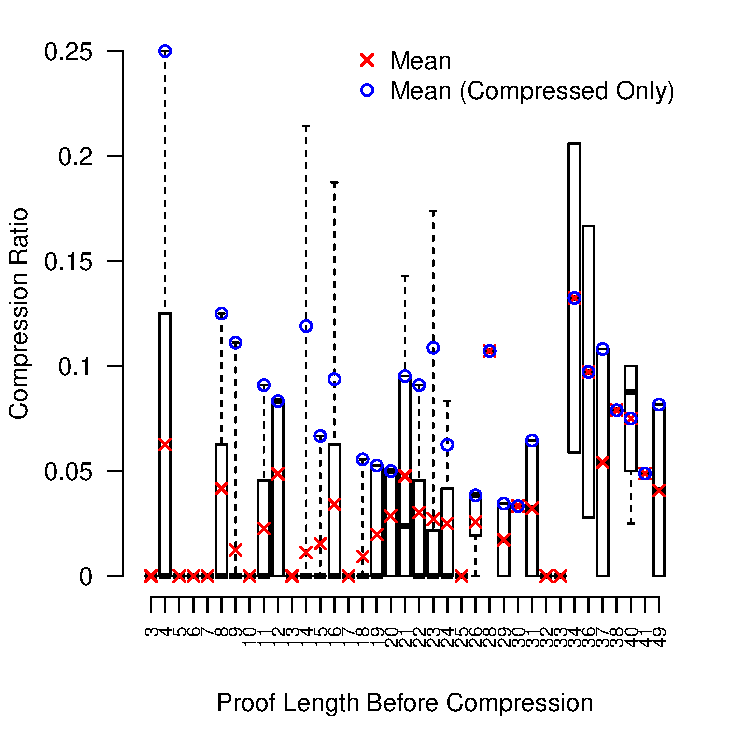
\includegraphics[scale=0.5]{images/compress_ratio_res_vs_proof_length_all_proofs.pdf} }}
    \subfloat[Number of (non-)compressed proofs]{{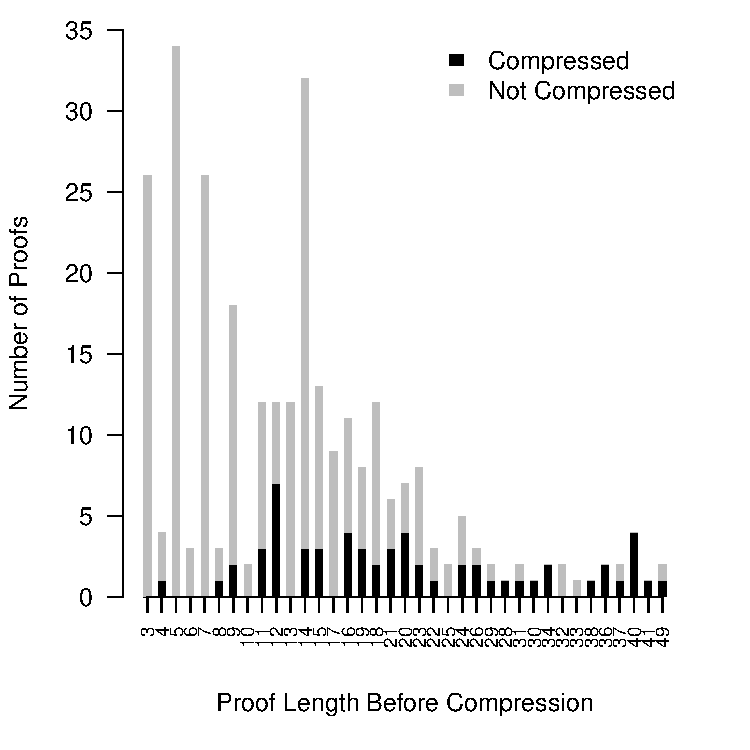
\includegraphics[scale=0.5]{images/num_compressed_stacked.pdf}}}\hfill
    \subfloat[Compressed length against input length]{{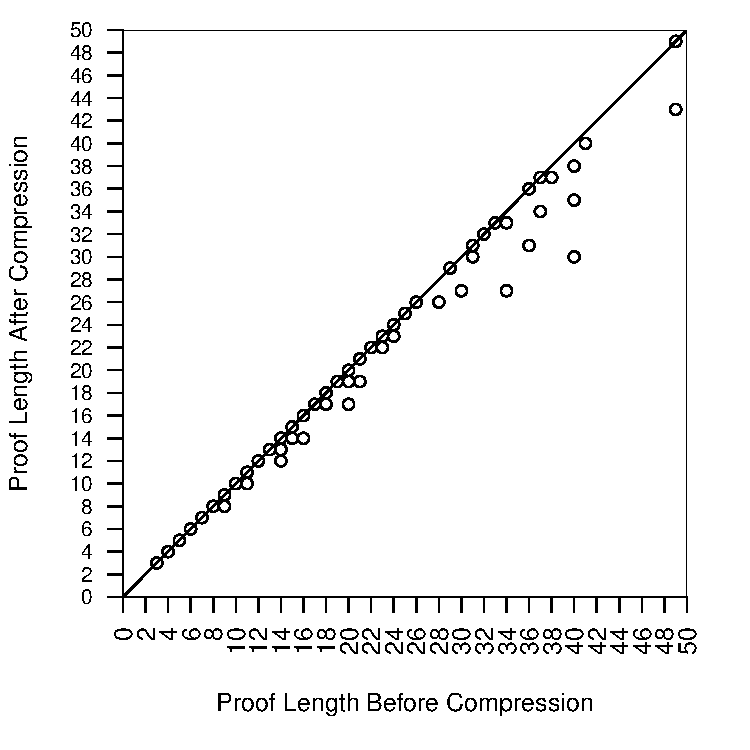
\includegraphics[scale=0.5]{images/compress_length_no_sub_vs_length_all_proofs.pdf} }}
    \subfloat[Cumulative proof lengths]{{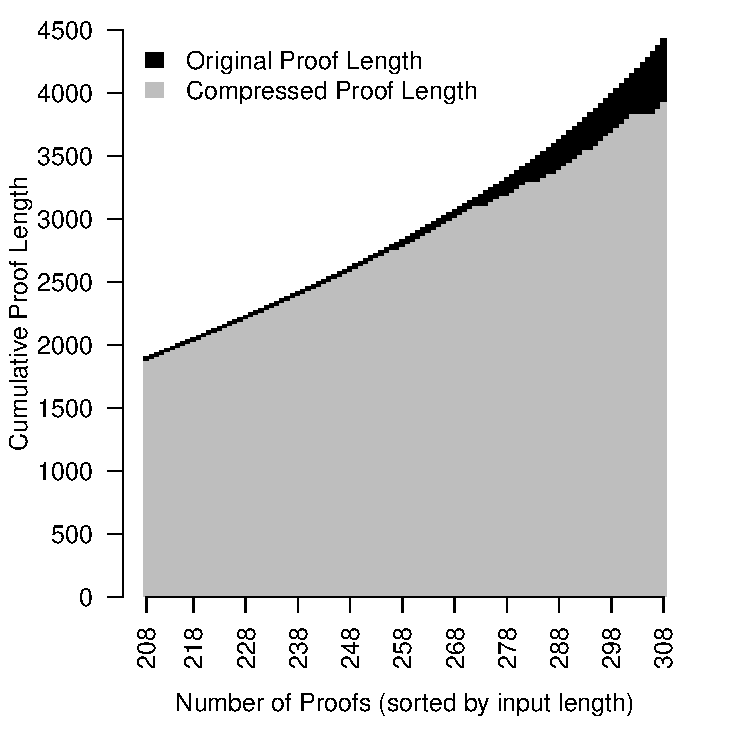
\includegraphics[scale=0.5]{images/cumulative_res_nodes_no_subs_top100.pdf}}}
\caption{Experimental results}
\label{fig:ex}

\end{figure}


\section{Conclusions and Future Work}


{\SFOLowerUnits} is our first attempt to lift a propositional proof compression algorithm to the first-order case. We consider it a prototype, useful to evaluate this approach. The results discussed in the previous section are encouraging, especially in comparison with existing results for the propositional case. In the near future, we shall seek improvements of this algorithm as well as other ways to overcome the difficulties related to the post-deletion unifiability property. The difficulties related to unit reintroduction suggest that other propositional proof compression algorithms that do not require reintroduction (e.g. {\RecyclePivotsIntersection} \cite{LURPI}) might need less sophisticated bookkeeping when lifted to first-order.

The efficiency and versatility of contemporary automated theorem provers depend on inference rules and techniques that go beyond the pure resolution calculus. The generalization of compression algorithms to support such extended calculi will be essential for their usability on a wider range of problems.


\bibliographystyle{plain}
\bibliography{biblio}


\end{document}


